\subsection{Overview}

In this section we present our digital sticky notes usecase and application. This application provides
a more real-world usage of our technologies versus the more abstract Cognitive Block World, though is
still simple enough to be readily understandable. This use-case was designed to be as analogous to the
traditional pen-and-paper design as possible, aiming just to replace the interfaces with digital equivalents
while retaining the usage model. First, there is a shared global screen, on which the digital notes can be placed
or removed. This screen is large enough to accomdidate several users standing in front of it at the same time,
and that the notes that are displayed on the wall are large enough to be read from a few feet away. To interact
with the wall, each user utilizes their cellphones to go to a specific URL in their browser. This webpage
asks for their name, and then they are free to begin. On their phone, a user is
first presented with buttons to create a new note and to pick a note up off the global screen. On hitting the
create note button, they are greeted with an interface to allow them to create a note, choose its color, etc.
Once they are satisfied with the content, they can click the button at the bottom of the UI to place the note.
This then opens their camera on their phone, showing the contents now on the screen, and the user then points
their camera to the part of the display they wish to place their note, clicking with their finger on their screen.

\begin{figure}
    \centering
    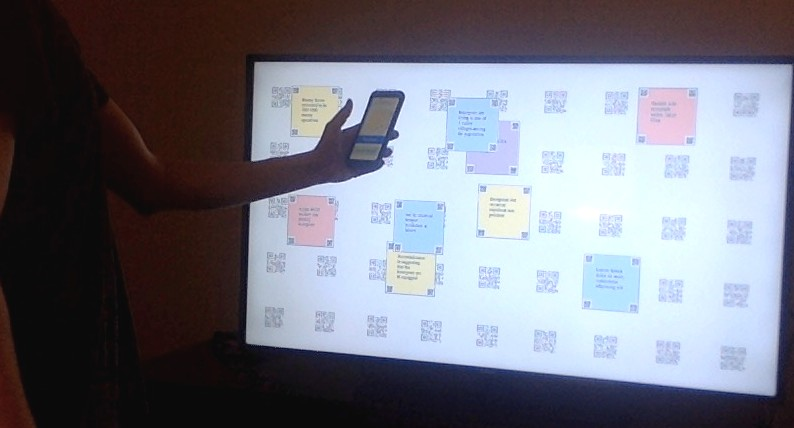
\includegraphics[width=0.45\textwidth]{figures/person_using}
    \caption{Someone using the sticky note application with their phone.}
      ~\label{fig:someone_using}
\end{figure}

